\chapter*{Introducción}
\addcontentsline{toc}{chapter}{\protect\numberline{}Introducción}
\label{chapter:Motivacion}

%Presentación
%Objetivo

%Motivación
Las propiedades f\'isicas de los materiales dependen en general del tamaño del sistema \cite{boverhof2015comparative}, por ejemplo, a escala nanom\'etrica ---de $1$ a $100$ nm \cite{boverhof2015comparative}---, la respuesta electromagn\'etica (EM) de bulto de los metales es menos relevante que los efectos de superficie \cite{zhao2008methods}.  La \emph{nanoplasm\'onica} estudia la respuesta EM a esta escala y el inter\'es en su estudio se ha renovado debido a las posibles aplicaciones que emplean las resonancias plasm\'onicas de superficie (Surface Plasmon Resonances, SPRs).  Áreas como la espectroscop\'ia \cite{novotny2006principles}, el sensado \cite{jain2008noble}, la litograf\'ia \cite{stockman2011nanoplasmonics}, y la biolog\'ia y  medicina \cite{jain2008noble}, son ejemplos del creciente interés en la nanoplasmónica. 


Otro ejemplo donde la nanoplasmónica ha impactado es en los \textit{biosensores} \cite{estevez2014trends,mun2015nanobiosensors}, definidos como ``dispositivos [$\ldots$] basados en elementos de reconocimiento biológico conectados a un transductor de señal, que relaciona la concentración de [uno o varios analítos] a una señal medible'' \cite{mun2015nanobiosensors}. Los biosensores se clasifican según el método de reconocimiento del analito, o bien, del transductor empleado \cite{mun2015nanobiosensors}. Dentro de los biosensores que ya se comercializan, los ópticos se caracterizan por su estabilidad, por sus mediciones sin marcadores, y por la  posibilidad de miniaturización y de multiplexeo \cite{estevez2014trends}, sobre todo los que se basan en nanoestructuras plasmónicas.

Los plasmones son oscilaciones colectivas de los electrones en un material metálico,  resultado del  acoplamiento con la radiaci\'on EM a las frecuencias donde ocurren las SPRs \cite{stockman2011nanoplasmonics}.  La clasificación de los plasmones comprende  dos tipos: propagantes y localizados.  Cuando los plasmones se propagan a lo largo de una interfaz plana entre un medio diel\'ectrico y uno met\'alico se denomina  \emph{plasm\'on-polarit\'on de superficie} (Surface Plasmon Polariton, SPP) \cite{maier2007plasmonics}.  Si el plasmón, en cambio, se encuentra en la superficie de una partícula  met\'alica, de tamaño finito, se le conoce como \emph{resonancia de plasm\'on de superficie localizado} (Localized Surface Plasmon Resonance, LSPR) \cite{maier2007plasmonics}.

Los biosensores ópticos emplean las SPRs por la respuesta que tienen ante cambios del índice de refracción de la matriz \cite{kabashin2009plasmonic}, que es el medio que rodea la estructura metálica.  Los sensores comerciales se caracterizan por el uso de SPPs \cite{estevez2014trends} en una configuración de reflexión total atenuada (Attenuated Total Reflection, ATR), en donde el índice de refracción del medio donde incide la luz que ilumina a la estructura metálica es mayor al de la matriz (ver Fig.  \ref{fig:ATR1}).  Las mediciones de reflectancia, en un sistema en configuración ATR, presentan mínimos para determinadas combinaciones de  ángulos de incidencia $\theta_i$ y longitud de onda $\lambda$  \cite{danilov2018ultra}.  Los sensores basados en las LSPRs se han propuesto como mejora sobre los sensores comerciales \cite{estevez2014trends}, ya que estos son al menos un orden de magnitud más sensibles a cambios de índice de refracción de la matriz  que los sensores basados en SPPs \cite{jain2008noble,kabashin2009plasmonic}. \\

	\begin{figure}[h!]\centering
	\begin{subfigure}{.05\textwidth}\vspace{-3.5cm}\caption{}\label{sfig:Pols}\end{subfigure}
	\begin{subfigure}{.43\textwidth} 
		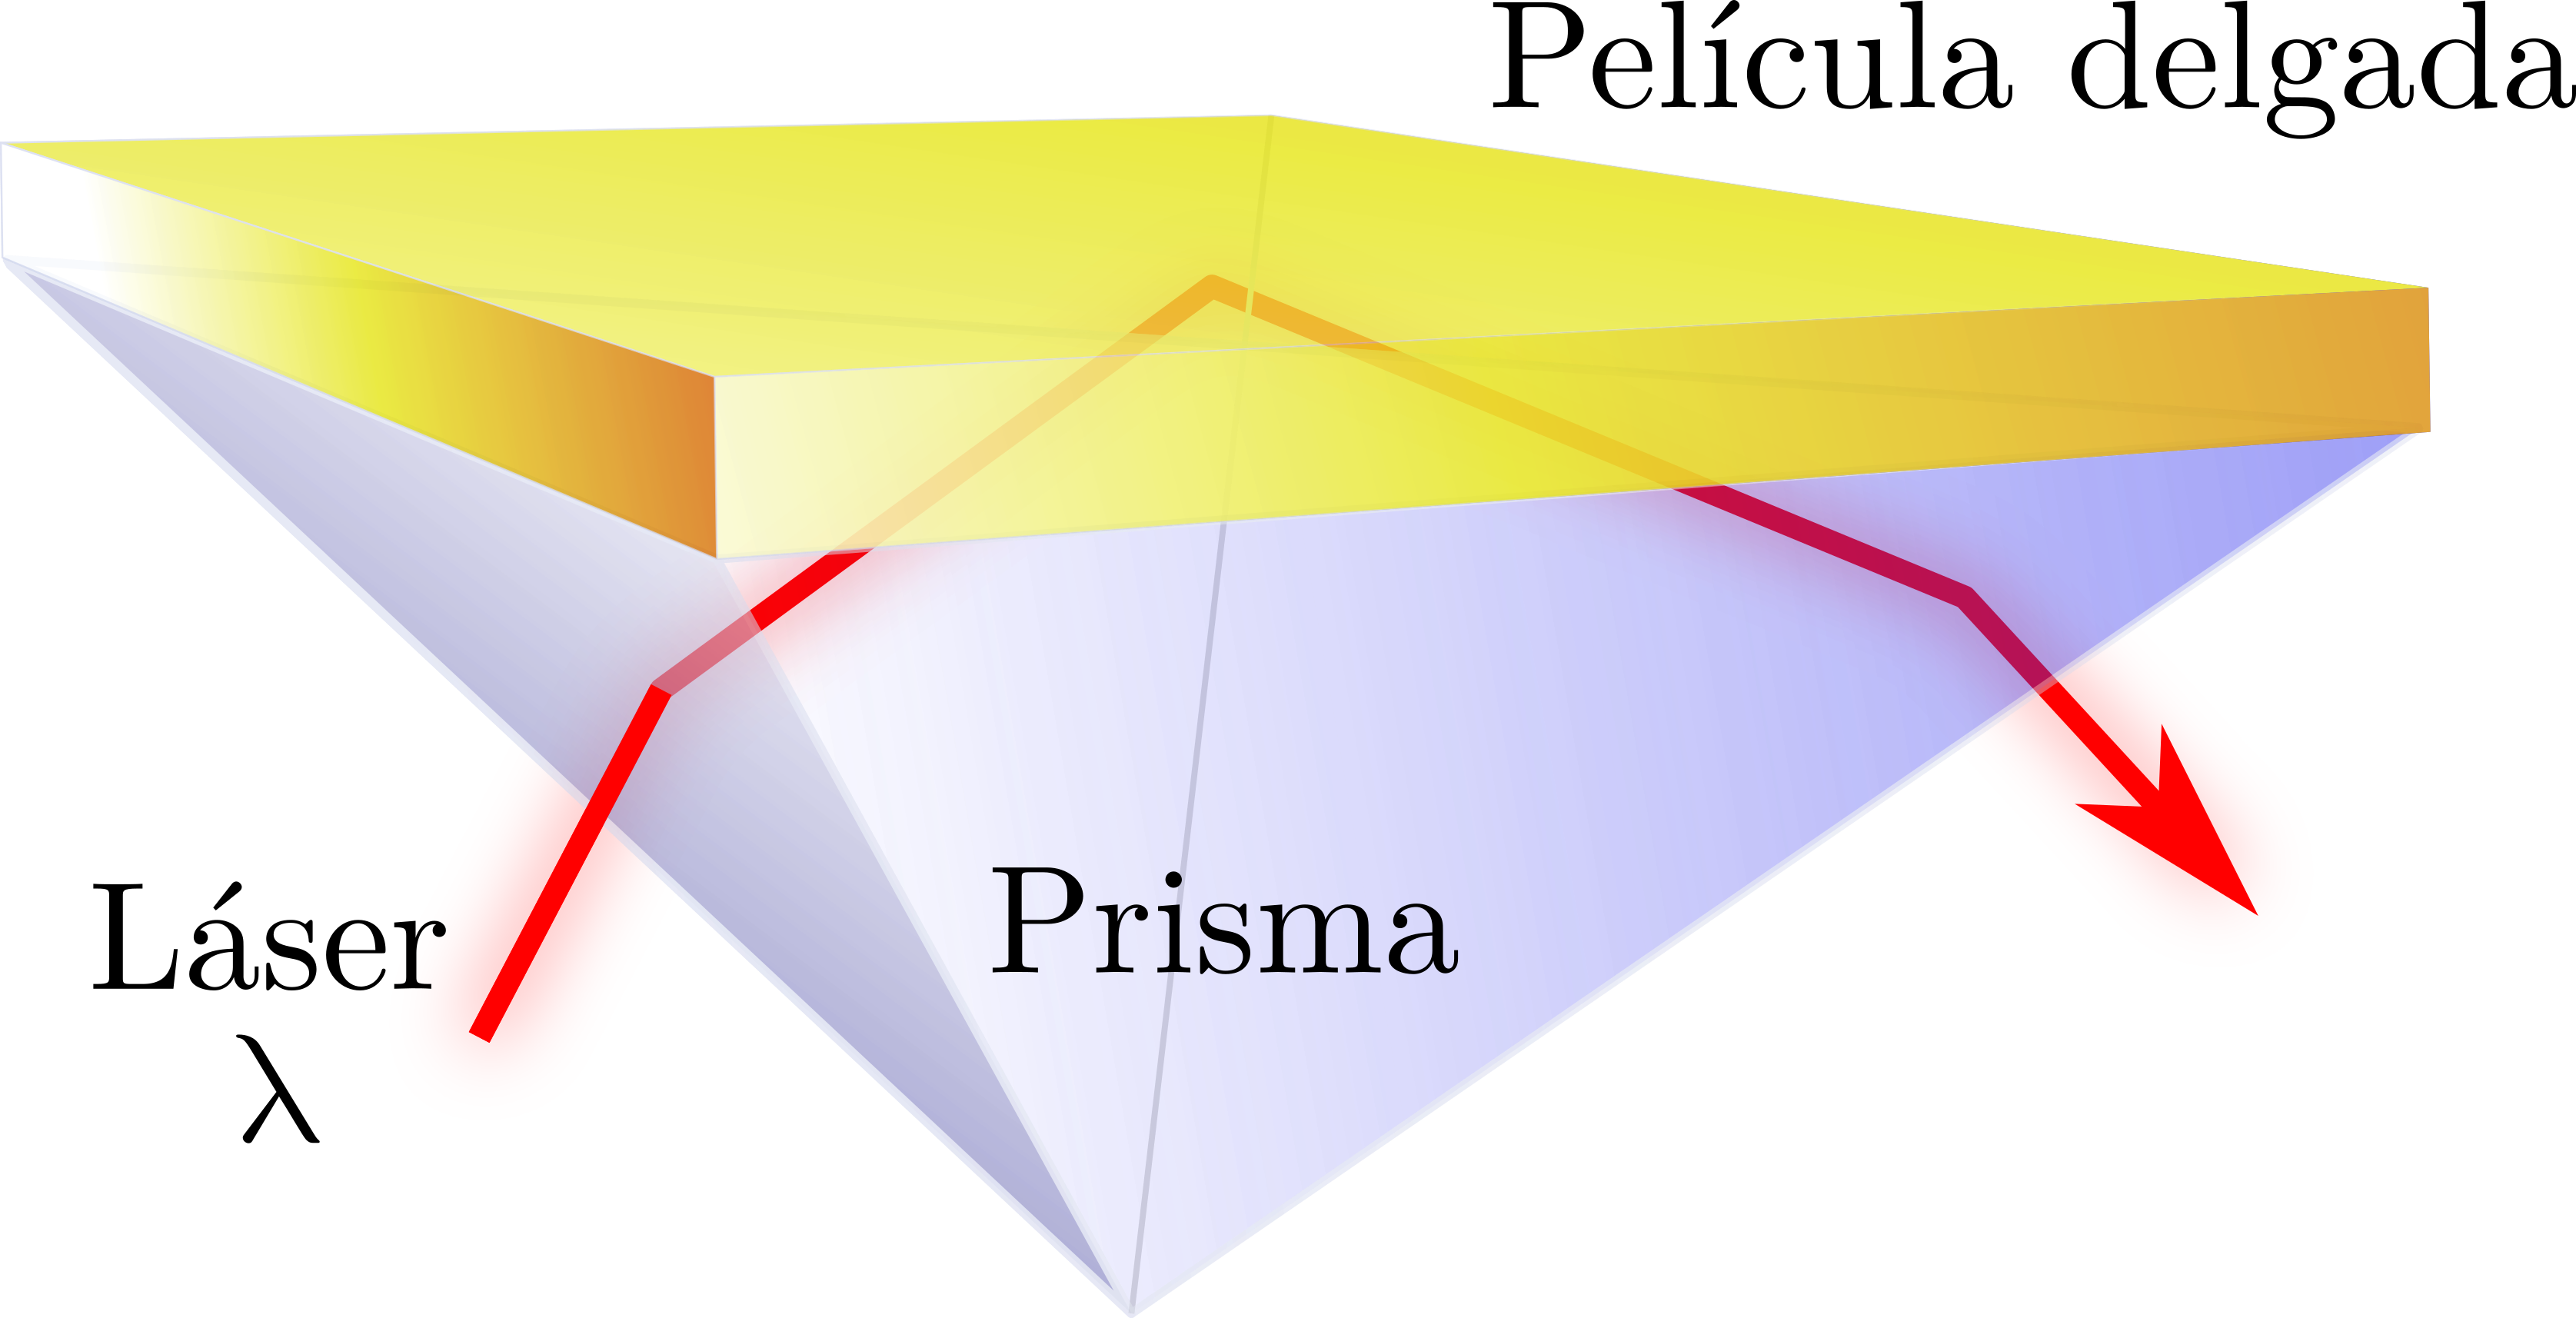
\includegraphics[scale=.225]{0-4-Introduccion/figs/SPP-3D.png}
		\end{subfigure}
	\begin{subfigure}{.05\textwidth}\vspace{-3.5cm}\caption{}\label{sfig:Polp}	\end{subfigure}
	\begin{subfigure}{.43\textwidth}  
		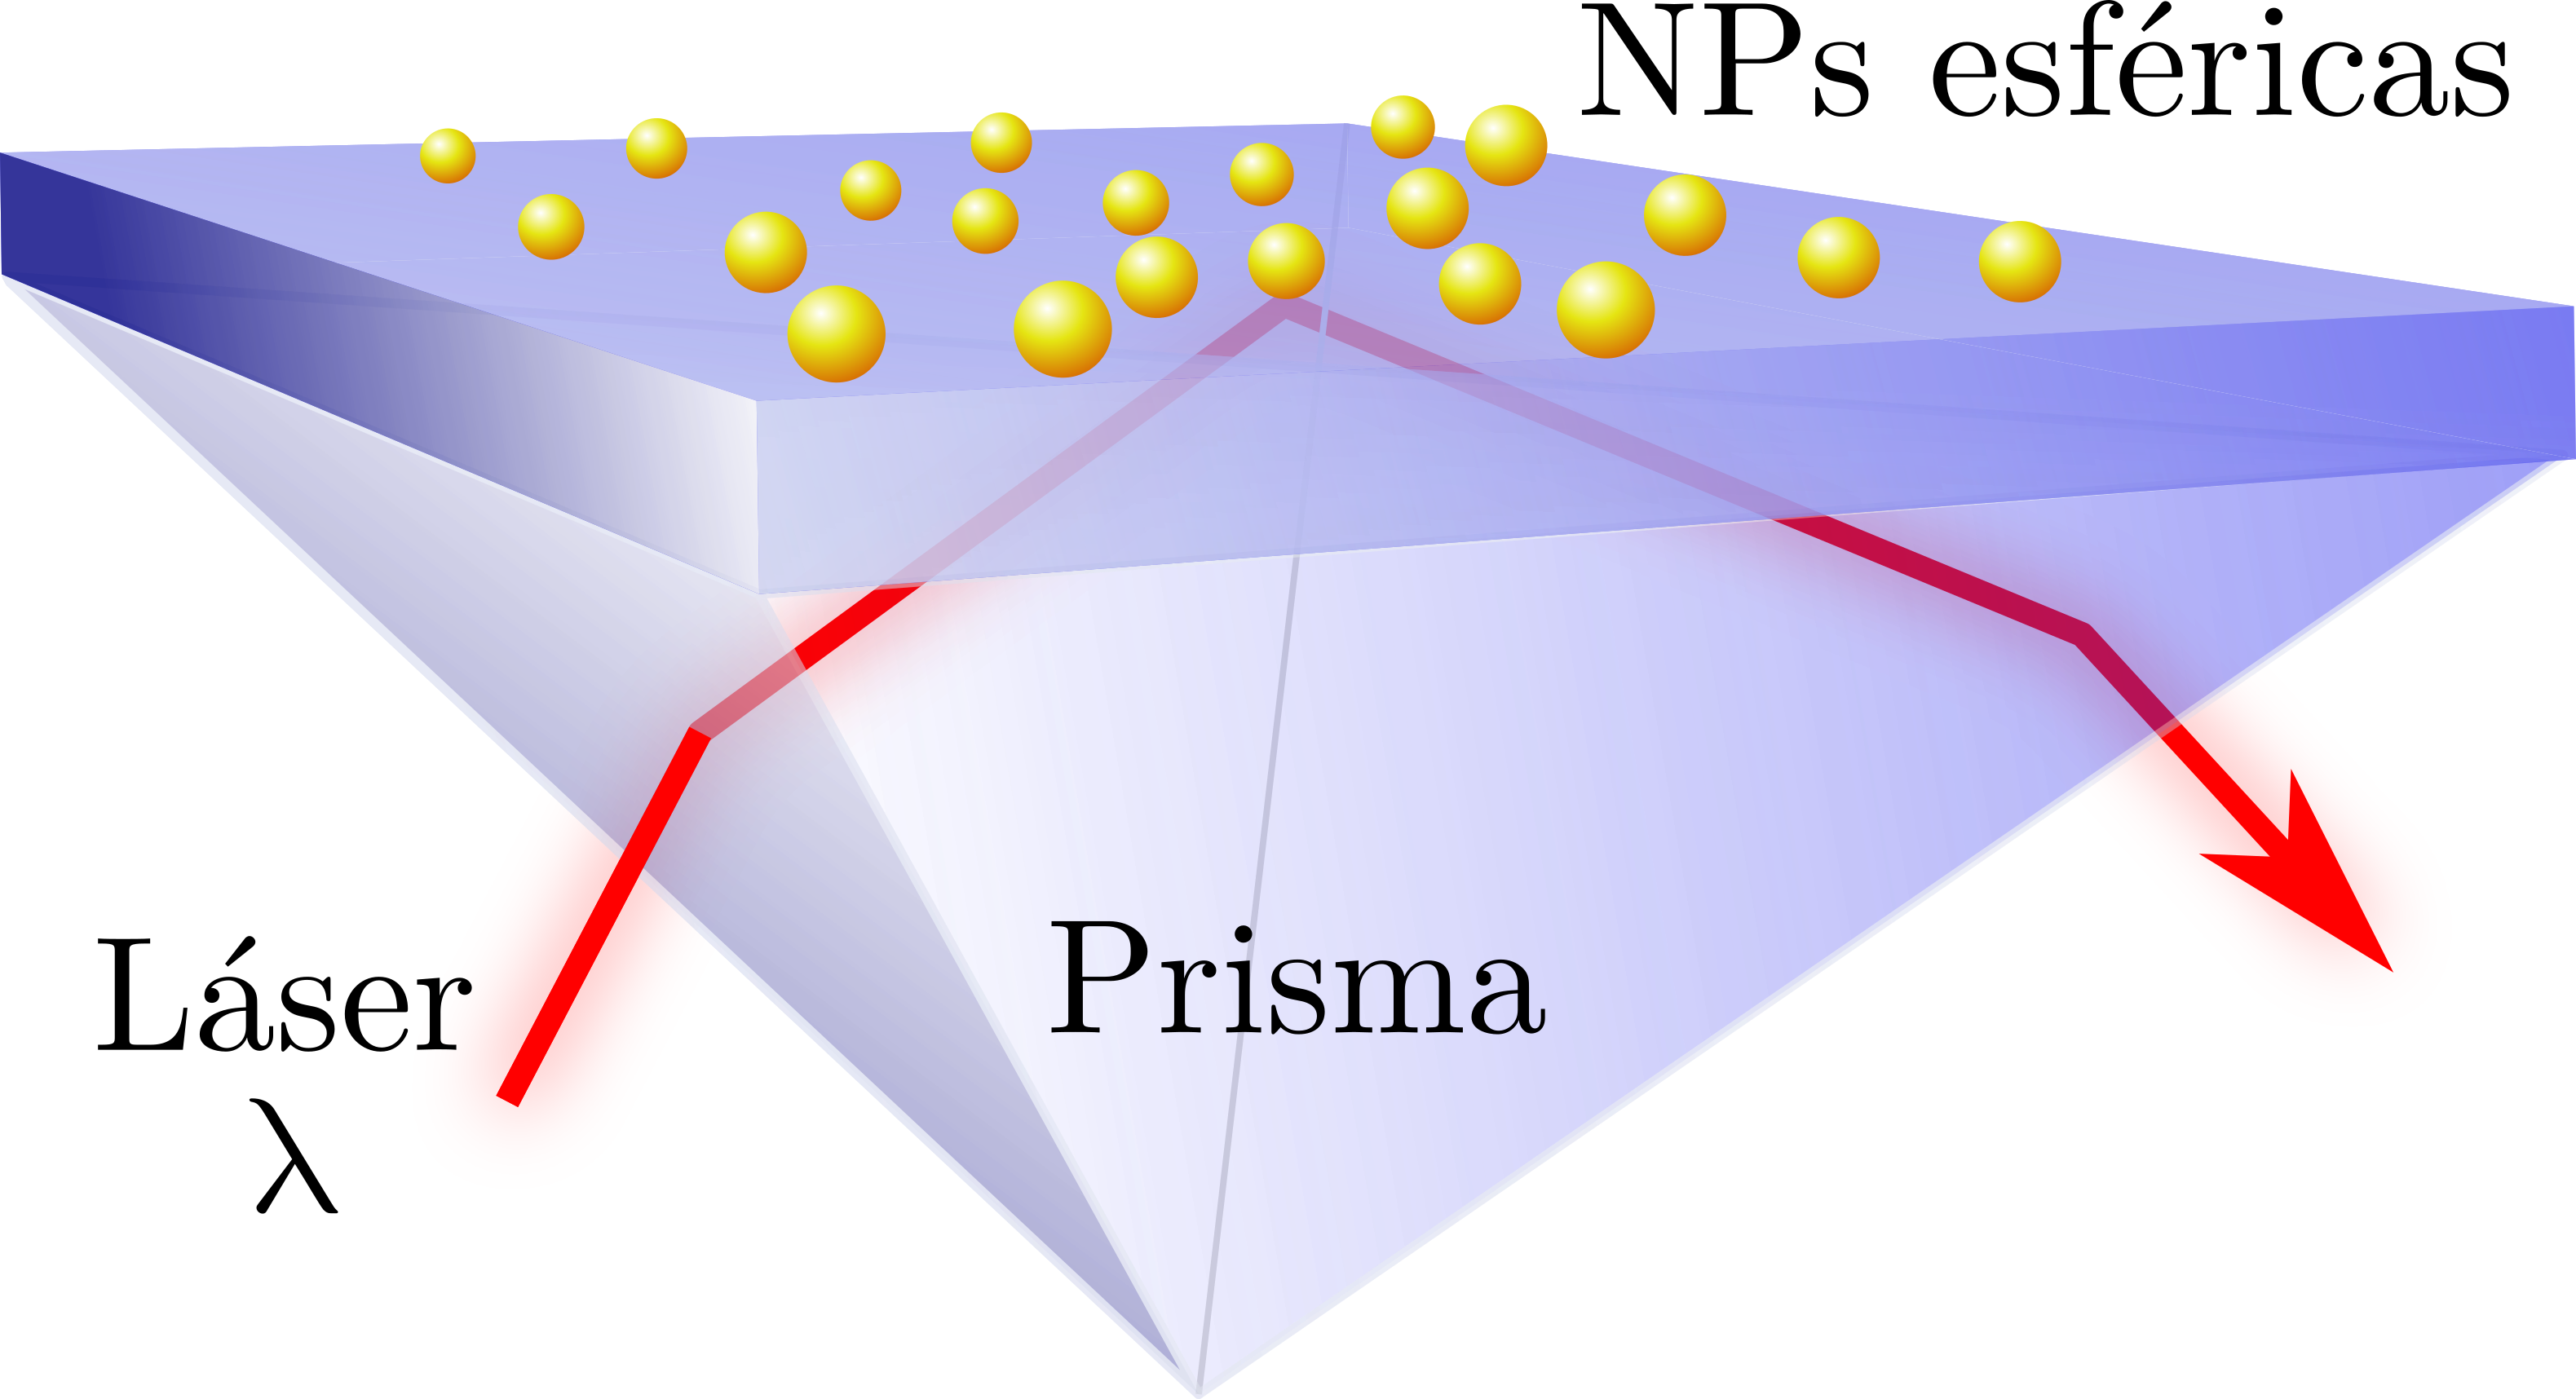
\includegraphics[scale=.225]{0-4-Introduccion/figs/NPs-3D.png}
	\end{subfigure} 
	\caption{ Iluminación de \textbf{a)} una película delgada y \textbf{b)} un arreglo de NPs esf\'ericas desordenánas por un haz de longitud de onda $\lambda$ a un \'angulo de incidencia $\theta_i$, en configuraci\'on ATR.}	\label{fig:ATR1}	
	\end{figure}	
	
En el 2009 se public\'o un art\'iculo \cite{kabashin2009plasmonic} en el que se propone un sistema bidimensional de NPs cilíndricas de oro, colocadas en arreglos periódicos, para la mejora en resoluci\'on  del biosensado [ver Fig. \ref{sfig:Nanocilindros}]; las dimensiones de los nanocilindros y el parámetro de red del arreglo son menores que la longitud de onda con la que se ilumina el arreglo \cite{kabashin2009plasmonic}.  En el artículo se reportó un modo plasmónico distinto a los modos normales de las NPs individuales, que permite el sensado del índice de refracción de la matriz y se le denominó \textit{modo guiado} \cite{kabashin2009plasmonic}.  En el 2018 se publicó que este modo es una respuesta colectiva del arreglo periódico \cite{danilov2018ultra} y depende del parámetro de red; en este artículo se le identificó como una \emph{resonancia de red del plasmón de superficie} (Plasmon Surface Lattice Resonance, PSLR), las cuales ocurren cuando un rayo difractado por la estructura periódica excita una LSPR en los elementos de la estructura \cite{vakevainen2013plasmonic}; las PSLR dependen del  ángulo de incidencia y de la periodicidad del arreglo \cite{danilov2018ultra}.  

En la Fig. \ref{sfig:DipATR} se grafican los cálulos de la reflectancia como función de la longitud de onda, para el arreglo mostrado en la Fig.  \ref{sfig:Nanocilindros}, en donde se supuso un sustrato de vidrio ($n=1.5$) y una matriz de aire ($n=1$), así como una monocapa de nanocilindros de $360$ nm de largo, $25$ nm de diámetro, con una separación entre ellos de $60$ nm. La respuesta EM del arreglo de nanocilindros   fue calculada al considerar a los cilindros como nanoesferoides y emplear una modificación del modelo de Maxwell Garnett \cite{atkinson2006anisotropic} ---que es una teoría de medio efectivo\footnote{Proceso de homogenización en donde se sustituye el medio heterogéneo por un medio continuo equivalente.  Este proceso se basa en la respuesta promedio del medio original cuando la longitud de onda de la luz incidente es grande en comparación a las dimensiones del sistema \cite{sihvola1999mixing}.}--- para la función dieléctrica efectiva de la monocapa $\varepsilon(\omega) = n^2 (\omega)$. En la Fig.\ref{sfig:k(w)Kobashin} se grafica la relación de dispersión  (energía como función de la  proyección perpendicular al sustrato del vector de onda)  del modo guiado (puntos blancos), mientas que en la Fig.  \ref{sfig:dLambda} se grafican los resultados experimentales del corrimiento al rojo del la PSLR al cambiar el índice de refracción de la matriz.

	\begin{figure}[h!]\centering
		\begin{subfigure}{.01\linewidth}\caption{ }\label{sfig:Nanocilindros} \vspace{5cm}	\end{subfigure}  
		\begin{subfigure}{.45\linewidth}\hspace*{-3em}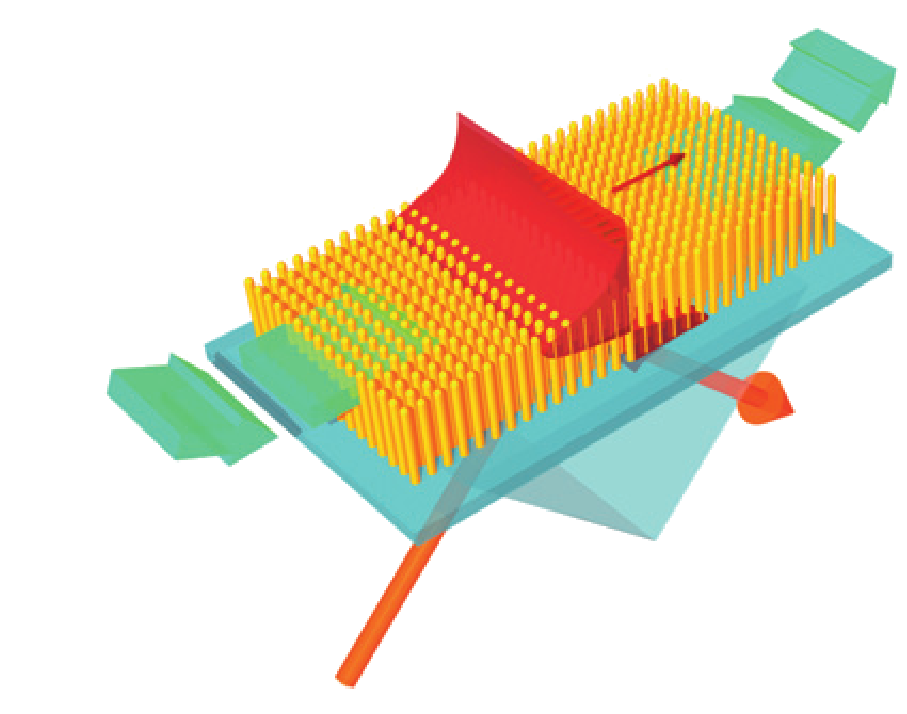
\includegraphics[scale=1]{0-4-Introduccion/figs/nanorods.png}\end{subfigure}
\begin{subfigure}{.01\linewidth}\caption{ }\label{sfig:DipATR}\vspace{4.75cm}\end{subfigure}  
		\begin{subfigure}{.45\linewidth}\hspace*{-1em}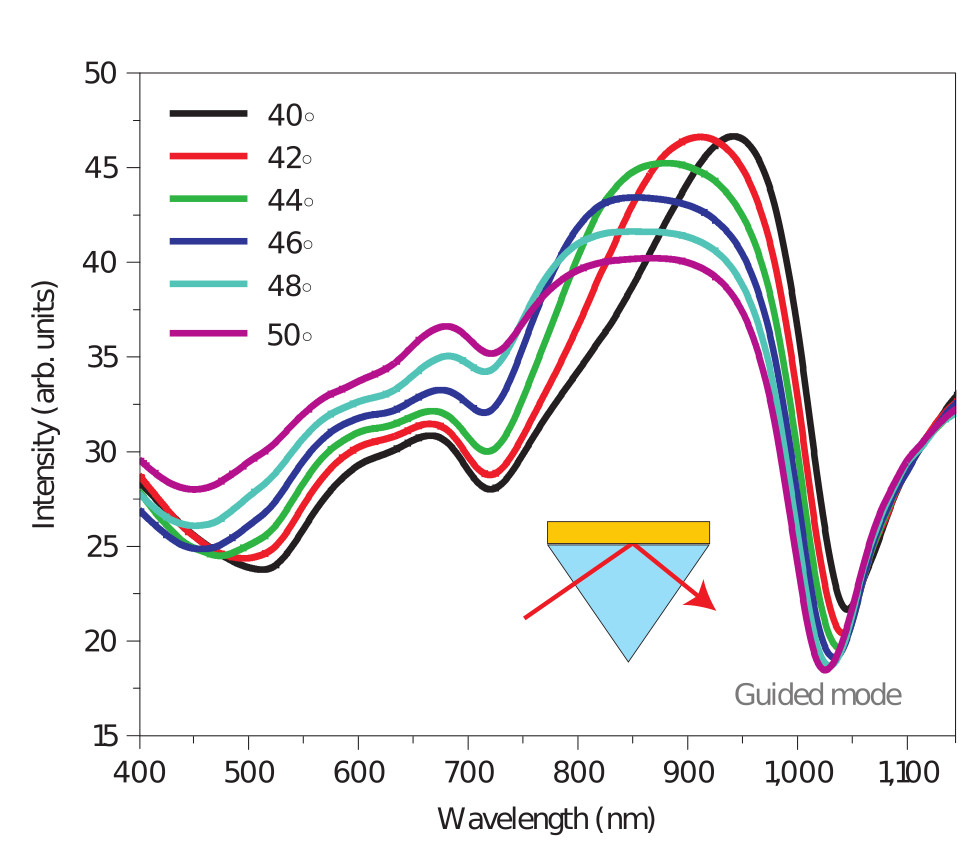
\includegraphics[scale=.9]{0-4-Introduccion/figs/reflectancia.png}\end{subfigure}\\
\begin{subfigure}{.01\linewidth}\caption{ }\label{sfig:k(w)Kobashin} \vspace{5cm}	\end{subfigure} 
		\begin{subfigure}{.45\linewidth}\hspace{1em}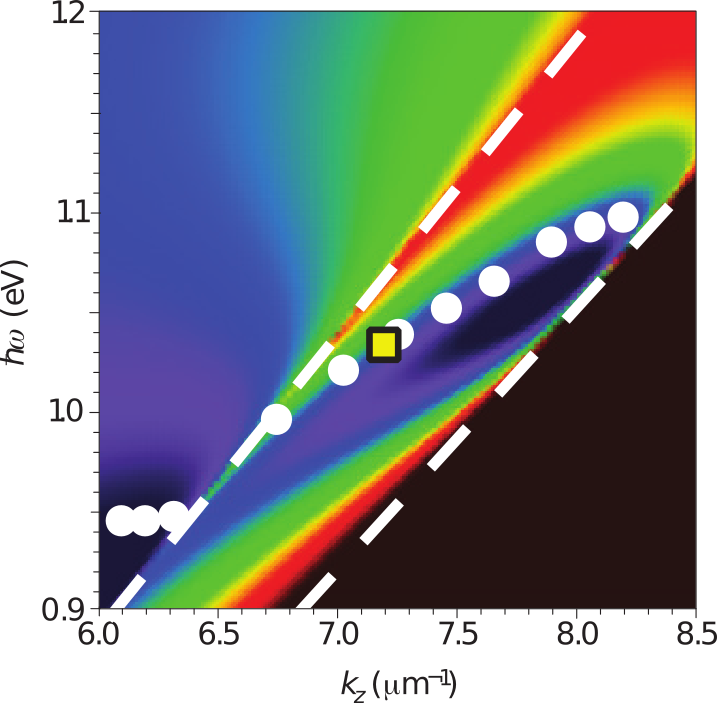
\includegraphics[scale=1]{0-4-Introduccion/figs/dispersion.png}\end{subfigure}	
\begin{subfigure}{.01\linewidth}\caption{ }\label{sfig:dLambda}\vspace{4.75cm}\end{subfigure}  
		\begin{subfigure}{.45\linewidth}\hspace*{-.5em}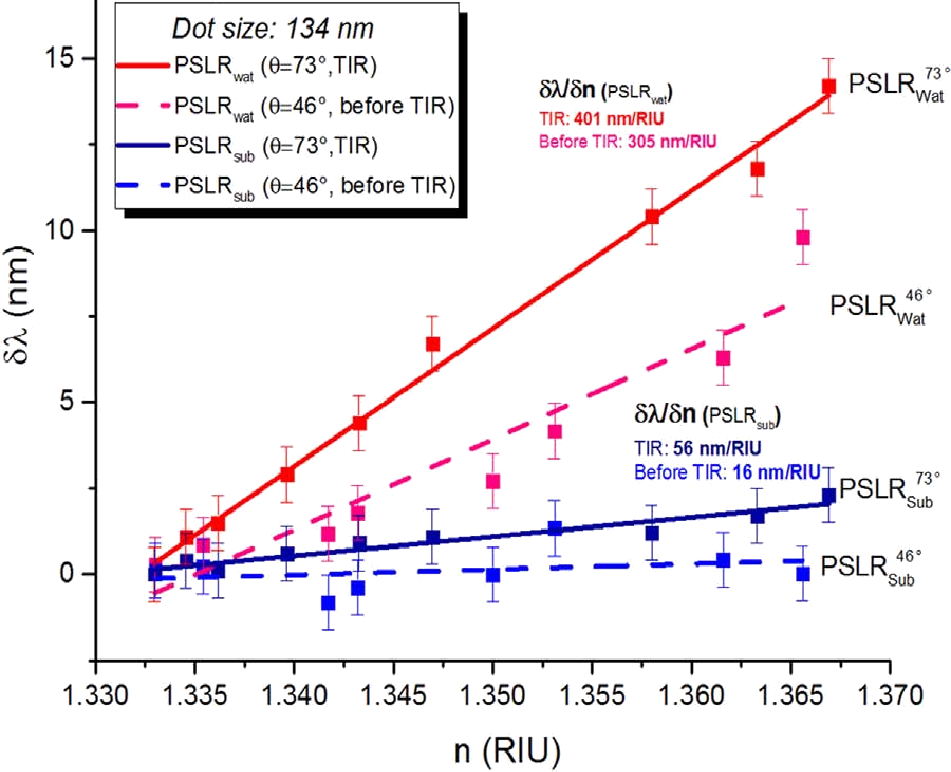
\includegraphics[scale=.9]{0-4-Introduccion/figs/sensibilidad.png}\end{subfigure}		
		\caption{\textbf{a)} Gráfica de la reflectancia  para un sistema periódico cuadrado de nanocilíndros de oro en ATR como función de la longitud de onda $\lambda$, para distintos ángulos de incidencia; y ) gráfica de la relación de dispersión  del arreglo  (extraídas de \cite{kabashin2009plasmonic}).  \textbf{c)} Gráfica de los parámetros elipsométricos (extraída de \cite{danilov2018ultra}) de un sistema de nanocilindros en un arreglo cuadrado periódico, en configuración ATR, en función de $\lambda$.  Las dimensiones de los nanocilindros en \textbf{a,b)} son $360$ nm de largo, $25$ nm de diámetro y una separación de $60$ nm entre ellos; los nanocilíndos están inmersos en una matriz de aire ($n=1$), sobre un sustrato de vidrio ($n=1.5$).  Las dimensiones de los nanocilindros en \textbf{c)} son $134$ nm de largo, y un parámetro de red de $320$ nm; la matriz y el sustrado empleados son los mismos que en \textbf{a)} y \textbf{b)}. }\label{fig:GraphsPapers}
	\end{figure}

Los cálculos de la reflectancia en ATR [Fig. \ref{sfig:DipATR}], muestran las resonancias plasmónicas típicas de NPs individuales para cilindros (modo longitudinal alrededor de $720$ nm y el transversal alrededor de $500$ nm) y adicional a ellas, se observa el modo guiado al rededor de los $1,050$ nm.  El modo guiado, al excitarse a energías menores del modo longitudinal, no puede ser una resonancia de NP individual y por tanto debe corresponder a un modo colectivo. En la Fig.  \ref{sfig:k(w)Kobashin} se grafica la relación de dispersión del modo guiado, donde los puntos blancos corresponden a los mínimos en la reflectancia alrededor de los $1,050$ nm de la Fig.  \ref{sfig:DipATR} del modo guiado.  Las líneas punteadas en la Fig.   \ref{sfig:k(w)Kobashin} corresponden a los ángulos críticos de las interfaces del medio efectivo simulado con el aire (línea izquierda superior) y con el sustrato (línea derecha inferior); la región oscura debajo de la línea punteada inferior derecha representa las combinaciones de energía y vector de onda sin sentido físico.  En la Fig.  \ref{sfig:dLambda} se muestran el corrimiento al rojo de de las PSLR cuando un haz de luz que incide a $75^\circ$ (líneas sólidas) y a $46^\circ$ (líneas punteadas) se difracta por la matriz de agua (líneas rojizas) y por el sustrato de vidrio (líneas azuladas). Dentro de la gráfica se muestran los valores de la sensibilidad $\delta \lambda /\delta n$ para cada caso.  

%\section*{Planteamiento del problema}

Las ventajas de un sistema ordenado como sensor son la posibilidad de ajuste del parámetro de red del sistema para optimizar la medición del sensor a la muestra, así como su posible compatibilidad con equipos comerciales actuales \cite{kabashin2009plasmonic}.  Sin embargo, la fabricaci\'on de arreglos ordenados de NPs presenta una complicaci\'on t\'ecnica de alto costo y largo tiempo de producción, por lo que se propone el uso de un arreglo bidimensional desordenado de NPs esféricas que presente una respuesta colectiva semejante a la reportada en \cite{kabashin2009plasmonic} y \cite{danilov2018ultra}.  Se ha observado que la respuesta colectiva en un arreglo desordenado también es sintonizable según las propiedades de las NPs empleadas, por lo que su uso en sensado no sólo cuenta con las ventajas de los sensores propuestos en \cite{kabashin2009plasmonic} y \cite{danilov2018ultra}, sino también una reducción en los precios y tiempos de producción. 

%\section*{Metodología}

Para  caracterizar la respuesta óptica de un arreglo bidimensional desordenado de NPs esféricas plasmónicas se emplea el modelo de esparcimiento coherente (Coherent Scattering Model, CSM) \cite{reyes2018analytical}, el cual proporciona expresiones analíticas para los coeficientes de amplitud de reflexión y de transmisión para una monocapa de NPs esféricas, idénticas, y desordenadas.  Las expresiones  dadas por el CSM dependen de las componentes de la matriz de esparcimiento empleada en la solución de Mie ---que resuelve los campos EMs esparcidos por una esfera iluminada por una onda plana \cite{bohren1998absorption}---, así como la respuesta EM del material que conforma las partículas esféricas de la monocapa: la función dieléctrica $\varepsilon(\omega)$.  Para caracterizar una excitación equivalente a la PSLR estudiada en \cite{kabashin2009plasmonic} y \cite{danilov2018ultra}, es decir, una respuesta colectiva apta para el biosensado, se calcula la reflectancia y transmitancia del sistema monocapa mediante los coeficientes de amplitud del CSM. 
 
Dado que el CSM emplea la respuesta EM del material que conforma a las NPs del arreglo, primero se consideró un modelo simple para caracterizar la respuesta de electrones libres dado por el modelo de Drude-Sommerfeld \cite{novotny2006principles} y, posteriormente, considerando materiales más  realistas, se emplearon funciones dieléctricas para el oro y la plata obtenidas de forma experimental \cite{johnson1972constants}, mostrados en la siguiente sección.  Después, se presenta la solución de Mie, que resuelve las ecuaciones de Maxwell para una partícula esférica, empleando la matriz de esparcimiento que relaciona los campos EMs esparcidos por la esfera con los campos EMs incidentes.  Por último, se presenta la deducción del CSM. 

%\section*{Contribuciones}
%\section*{Estructura de la tesis}
